\documentclass[letterpaper,10pt]{examdesign}
\usepackage[utf8]{inputenc}
\usepackage{amsmath}
\usepackage{amsfonts}
\usepackage{amssymb}
\usepackage[spanish,es-noshorthands]{babel}
\usepackage[T1]{fontenc}
\usepackage{lmodern}
\usepackage{graphicx,hyperref}
\usepackage{tikz,pgf}
\usepackage{subfig}
\usepackage{wrapfig}
\usepackage{multicol}
\usepackage[includeheadfoot,left=0.4in,right=0.4in,top=0.3in,bottom=0.2in]{geometry}
%\NumberOfVersions{3}
\ShortKey
\class{
\includegraphics[height=1.7cm]{Images/logo-colegio.png} Cálculo $9^{\circ}$}
\examname{Prueba bimestral 1}
\def\namedata{Nombre: \hrulefill \\[10pt]
Curso: \hrulefill \\[10pt]
Fecha: \hrulefill}
\begin{document}
\begin{multiplechoice}[rearrange=no,keycolumns=4,examcolumns=2]
\begin{block}
RESPONDE LAS 2 PREGUNTAS SIGUIENTES DE ACUERDO CON EL SIGUIENTE
GRÁFICO\\
Sigue estrictamente el orden de las operaciones indicadas y verás que siempre llegas al mismo resultado.
\hspace*{1cm}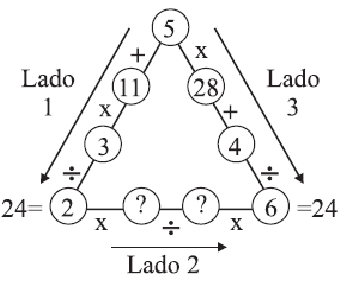
\includegraphics[scale=.55]{Images/triangulonum.png}
\begin{question}
Los números que al ubicarse en el Lado 2 NO cumplen con la condición requerida para que el resultado final sea 24 son, respectivamente
\choice{4 y 2}
\choice{16 y 8}
\choice[!]{22 y 16}
\choice{26 y 13}
\end{question}
\begin{question}
Los números que aparecen dentro de los círculos del Lado 1, pertenecen al conjunto de los números
\choice{impares}
\choice[!]{primos}
\choice{pares}
\choice{enteros positivos}
\end{question}
\end{block}
\begin{block}
\begin{question}
Observa los siguientes triángulos; 
Sabiendo que los triángulos son semejantes y la medida de sus lados son proporcionales, entonces el valor de $a$ es:
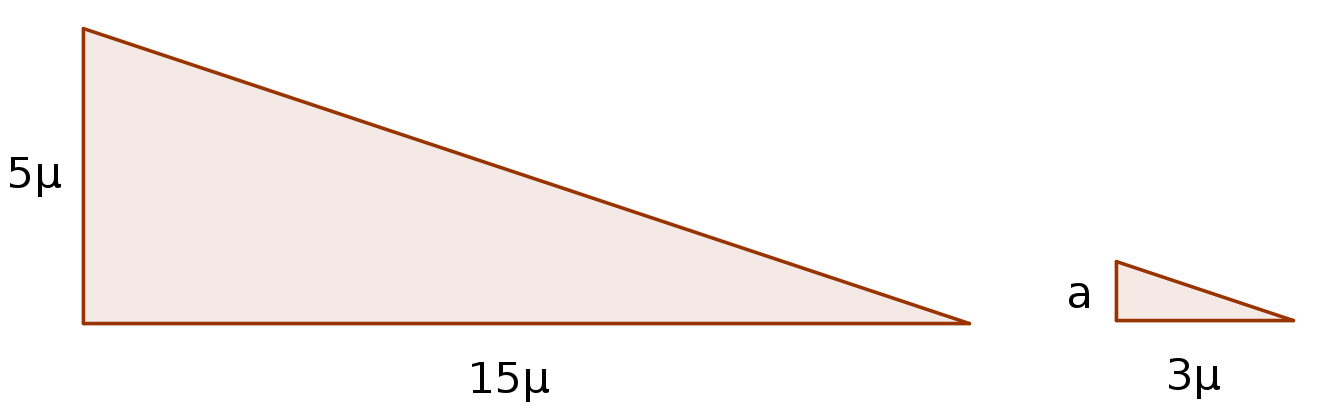
\includegraphics[scale=.75]{Images/semajanza01.png} 
\choice[!]{1}
\choice{3}
\choice{5}
\choice{15}
\end{question}
\end{block}
\begin{block}
RESPONDE LAS DOS PREGUNTAS QUE SIGUEN DE ACUERDO CON LA SIGUIENTE INFORMACIÓN\\
De un tanque lleno de agua, con capacidad de 400 litros, se extrae 1/5  de agua el día lunes, 1/4 del agua restante el día martes y 9/30 del agua que queda en el tanque el día miércoles.
\begin{question}
La menor cantidad de agua se sacó el día
\choice{lunes}
\choice{martes}
\choice[!]{miércoles}
\choice{en los tres días se extrajo la misma cantidad de agua}
\end{question}
\begin{question}
¿Qué cantidad de agua queda disponible para el día jueves?
\choice{100 litros}
\choice[!]{168 litros}
\choice{175 litros}
\choice{232 litros}
\end{question}
\end{block}
\begin{question}
Si 48 de los 60 asientos en un autobús estaban ocupados, ¿qué porcentaje de los asientos NO estaba ocupado?
\choice{12\%}
\choice[!]{20\%}
\choice{25\%}
\choice{60\%}
\end{question}
\begin{question}
¿Cuál de las siguientes fracciones NO es igual a $\dfrac{36}{45}$?
\choice{$\frac{4}{5}$}
\choice{$\frac{12}{15}$}
\choice[!]{$\frac{24}{35}$}
\choice{$\frac{48}{60}$}
\end{question}
\begin{block}
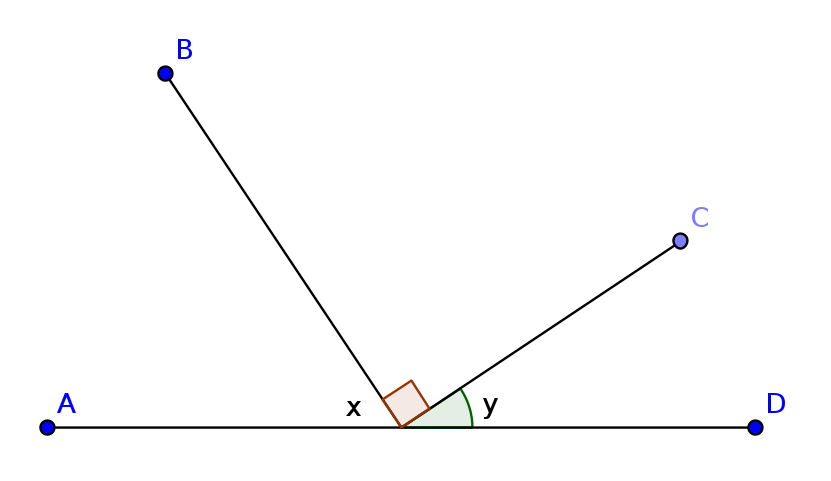
\includegraphics{Images/angulosxy.png} 
\begin{question}
En la figura de arriba, ¿cuál es el valor de $x+y$?
\choice{30}
\choice{45}
\choice{110}
\choice[!]{90}
\end{question}
\end{block}
\begin{question}
¿Cuál de los siguientes es igual a $25(27+29+31)$?
\choice{$25(27+29)+31$}
\choice{25(27)+29+31}
\choice[!]{25(27)+(29+31)(25)}
\choice{25+(27)(29)(31)}
\end{question}
\begin{question}
Al efectuar $\dfrac{7}{5}\times \left(\dfrac{3}{7}-\dfrac{2}{5}\right)=$ \; se obtiene
\choice{$\frac{1}{165}$}
\choice{$\frac{1}{35}$}
\choice[!]{$\frac{1}{25}$}
\choice{$\frac{19}{15}$}
\end{question}
\begin{question}
Un closet contiene 24 pares de zapatos. Si el 25\% de esos pares de zapatos son negros, ¿cuántos pares NO son negros?
\choice{4}
\choice{6}
\choice{12}
\choice[!]{18}
\end{question}
\begin{block}
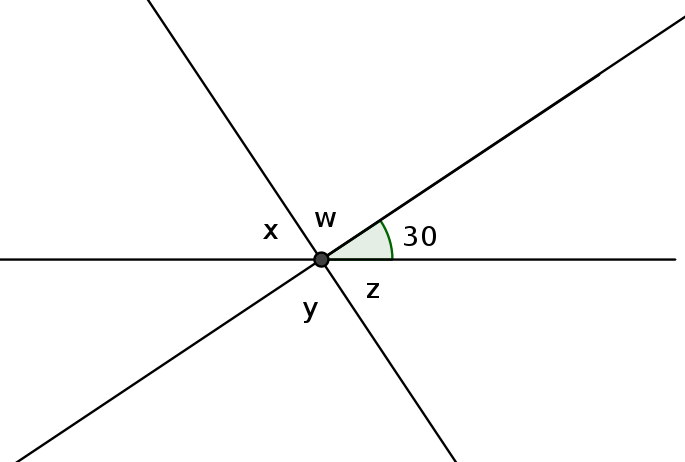
\includegraphics[scale=1.1]{Images/anguloswxyz.png} 
\begin{question}
En la figura anterior, $w+x+y+z=$
\choice[!]{330}
\choice{300}
\choice{270}
\choice{240}
\end{question}
\end{block}
\begin{block}
\hspace*{.5in}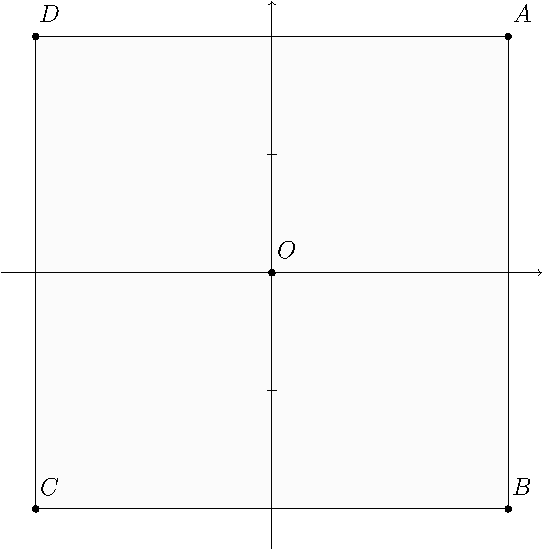
\includegraphics[scale=.75]{Images/cuadrado.pdf}
\begin{question}
En la figura de arriba, ABCD es un cuadrado con centro en el origen. Si las coordenadas del vértice A son (4,4), ¿cuáles con las coordenadas del vértice C?
\choice{$(-4\sqrt{2},-4\sqrt{2}$}
\choice{$(-4\sqrt{2},-4$}
\choice[!]{$(-4,-4)$}
\choice{$(-4,4)$}
\end{question}
\end{block}
\begin{question}
De dos varillas cuyas longitudes son 360 cm y 108 cm, respectivamente, se desea obtener trozos iguales que tengan la longitud máxima posible. El mayor número total de trozos obtenidos es
\choice[!]{13} \choice{12} \choice{18} \choice{16}
\end{question}
\begin{block}
\hspace*{1cm}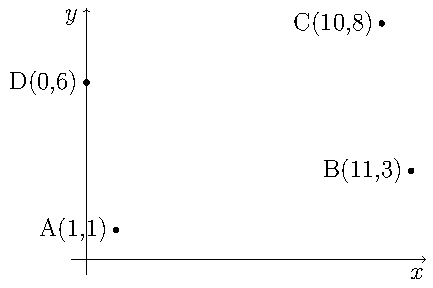
\includegraphics[scale=.8]{Images/puntos.pdf} 
\begin{question}
Si se trasladan los cuatro puntos 5 unidades a la izquierda y 2 unidades hacia arriba, las coordenadas de los nuevos puntos serán, respectivamente
\choice[!]{$(-4,3), (6,5), (5,10), (-5,8)$}
  \choice{$(6,-1), (16,1), (15,6), (5,4)$}
  \choice{$(-4,-1), (6,1), (5,6), (-5,4)$}
  \choice{$(6,3), (16,5), (15,6), (-5,4)$}
\end{question}
\end{block}
\begin{question}
Un rectángulo tiene 5,97 metros de largo y 8 metros de ancho. ¿Cuál de los siguientes valores es más cercano al área de este rectángulo?
\choice{$46\,m^{2}$}
\choice[!]{$ 48\;m^2 $}
\choice{$ 50\;m^2 $} 
\choice{40 $ m^2 $}
\end{question}
\begin{question}
A una función del Teatro Infantil entraron 270 personas. Por cada dos niños entró un adulto a la función. Cada adulto pagó \$6.000 y los niños entraron gratis. ¿Cuanto dinero se recaudó?
\choice{\$810\,000} \choice[!]{\$540\,000}  \choice{\$1'080\,000} \choice{\$1'620\,000}
\end{question}
\begin{block}
Dados los conjuntos $A=\{2,3,5\}$ y $B=\{1,2,3,4\}$,
\begin{question}
el producto cartesiano $A\times B$ ser\'{a}:
\choice{\{(1,2), (1,3), (1,5), (2,2), (2,3), (2,5), (3,2), (3,3), (3,5), (4,2), (4,3), (4,5)\}}
\choice{\{(2,2),(3,3),(5,5)\}}
\choice[!]{\{(2,1), (2,2), (2,3), (2,4), (3,1), (3,2), (3,3), (3,4), (5,1), (5,2), (5,3), (5,4)\}}
\choice{\{(1,2), (2,3), (3,4), (3,5)\}}
\end{question}
\begin{question}
La relación $R=\{(x,y)\,/\, x\in A,\, y\in B, \text{ y } y=x-1 \} $ está constituída por:
\choice{\{(2,1), (3,2), (4,3), (5,4)\}}
\choice{\{(1,2), (2,3), (3,4), (4,5)\}}
\choice{\{(1,1), (2,2), (3,3), (4,4), (5,5)\}}
\choice[!]{\{(2,1), (3,2), (5,4)\}}
\end{question}
\end{block}
\end{multiplechoice}
\end{document}
